 \documentclass[12pt]{article}
%\usepackage[portuguese]{babel}
\usepackage{natbib}
\usepackage{url}
\usepackage[utf8x]{inputenc}
\usepackage{amsmath}
\usepackage{graphicx}
\graphicspath{{images/}}
\usepackage{parskip}
\usepackage{fancyhdr}
\usepackage{vmargin}
\setmarginsrb{1.5 cm}{2.5 cm}{1.5 cm}{2.5 cm}{1 cm}{1.5 cm}{1 cm}{1.5 cm}
\usepackage{hyperref}
\hypersetup{
    colorlinks=true,
    citecolor=black,
    filecolor=black,
    linkcolor=black,
    urlcolor=black
}
\let\oldhref\href
\renewcommand{\href}[2]{\oldhref{#1}{\bfseries#2}}

\usepackage[bottom]{footmisc}
\usepackage{caption}
\DeclareCaptionFormat{sanslabel}{#3}%
\usepackage[section]{placeins}
\usepackage{xcolor}
\definecolor{light-gray}{gray}{0.95}
\usepackage{listings}
\lstset{basicstyle=\ttfamily,
  showstringspaces=false,
  commentstyle=\color{red},
  keywordstyle=\color{blue},
  backgroundcolor=\color{light-gray},
  breaklines=true,
  extendedchars=true,
  basicstyle=\small,
  literate={é}{{\'e}}1
}
\lstset{aboveskip=15pt,belowskip=15pt}
\usepackage[autostyle]{csquotes}  
\def\labelitemi{--}
\usepackage{enumitem}
\setlist{nosep}
\usepackage{booktabs}

\title{Tutorial git}								% Title
%\author{}								% Author
\date{\today}											% Date

\makeatletter
\let\thetitle\@title
%\let\theauthor\@author
\let\thedate\@date
\makeatother

\pagestyle{fancy}
\fancyhf{}
%\rhead{\theauthor}
\lhead{\thetitle}
\cfoot{\thepage}

\begin{document}

%%%%%%%%%%%%%%%%%%%%%%%%%%%%%%%%%%%%%%%%%%%%%%%%%%%%%%%%%%%%%%%%%%%%%%%%%%%%%%%%%%%%%%%%%

\begin{titlepage}
	\centering
    \vspace*{0.5 cm}
    
\includegraphics[scale = 0.3]{resources/logo4.png}\\[1.0 cm]
    \textsc{\LARGE \newline\newline UNIX 101}\\[2.0 cm]
	\textsc{\Large or "How to feel like a true hack3r"}\\[0.5 cm]
	\rule{\linewidth}{0.2 mm} \\[0.4 cm]
	{ \huge \bfseries \thetitle}\\
	\rule{\linewidth}{0.2 mm} \\[1.5 cm]
	
%	\begin{minipage}{0.5\textwidth}
%		\begin{flushleft} \large
%			\emph{Professor:}\\
%			Renan E P Lima\\
%            Departamento de Matemática\\
%			\end{flushleft}
%			\end{minipage}~
%			\begin{minipage}{0.4\textwidth}
%           
%			\begin{flushright} \large
%			\emph{Grupo:} \\
%			Gabriel P Crestani\\
%           Victor R Sales\\
%		\end{flushright}
%        
%	\end{minipage}\\[2 cm]
	
	
    \thedate
    
    
    
	
\end{titlepage}

%%%%%%%%%%%%%%%%%%%%%%%%%%%%%%%%%%%%%%%%%%%%%%%%%%%%%%%%%%%%%%%%%%%%%%%%%%%%%%%%%%%%%%%%%

\tableofcontents
\pagebreak

%%%%%%%%%%%%%%%%%%%%%%%%%%%%%%%%%%%%%%%%%%%%%%%%%%%%%%%%%%%%%%%%%%%%%%%%%%%%%%%%%%%%%%%%%

\section{Foreword}

\subsection{Objective}
This tutorial should teach you the basics of working with git.
It will demonstrate what one can perform with this tool, how it works and how to use it.

If you work thoroughfully, at the end of this tutorial, you should know:

\begin{itemize}
\item What is git
\item Why it is important to know how to use git
\item How to generate a SSH key and how to use SSH to communicate with a git server
\item How to clone a remote repository
\item How to contribute to a repository
\end{itemize}


\subsection{Preliminary setup}

You are going to need a UNIX-like operating system for this tutorial.
A Linux distribution is preferred but a Mac can also do the job (OS X is a variant of FreeBSD).

You need the git binary to be installed on your system. If you have finished the first tutorial, you should know how to install it\footnote{Check that it is installed with \texttt{which git}; if it is not, install it with \texttt{sudo apt install git}. If you had trouble with that, take some time to read again the previous tutorial}.

Lastly, you need to configure git:

\begin{lstlisting}[language=bash]
$git config --global user.name "Firstname Lastname" # Put your own name here and do not forget the quotes!
$git config --global user.email firstname.lastname@mail.com # Put your own name and email here
\end{lstlisting}

The configuration will be saved in your home, in the hidden file \texttt{.gitconfig}. This is where git will look for user configuration, by default. Use \texttt{cd} and \texttt{cat .gitconfig} to see the file content. Confirm that the informations you entered earlier are correct.

\section{Git}

\subsection{The why: problems, problems, problems}

Because a coding project contains a lot of files of different type (code files, generated files, libraries, documentation, etc), working alone or collaborating on one proves itself to be complicated without some kind of versioning or collaboration tool.

Imagine having to share your work with colleagues throught USB keys or some cloud drive drag\&drop operations. Then imagine working all at the same time on the same project. How to handle conflicts? Regressions? What if you submit some work but your colleague was about to do the same and you modified the same files? What if you somehow loose your work? How do you restore it?

These problems are bound to happen with a team of one or two persons and it is already a pain. Now imagine the same problems for a team of ten (or more) persons working on the same project. That is \textbf{a lot} of pain.

\subsection{The what: Version Control System}

Hopefully, smart people have worked on that problem for us, years ago. Version Control Systems (VCS) help solve some of these issues. Technically, there exist multiple VCS but \href{https://git-scm.com/}{git} has become the de facto choice in the last ten years. Git is basically a tool that allows one to keep an history of files. It has the particularity to be distributed: multiple persons can keep a common history of files.

Thanks to git, you will be able to:

\begin{itemize}
\item Backup easily and whenever you want your work
\item Prevent accidents (e.g. unwanted file or content deletion)
\item Browse the history of your modifications and come back to some point in time if necessary
\item Work collaboratively on a project
\item ...and much more!
\end{itemize}


\subsection{The why you should really really learn using git}

Just to highlight the popularity of these kind of tools, one needs to understand that \textbf{every single serious software company in the world uses a VCS} and most of them rely on git. All professional software engineers are expected to know how to use this tool. Not only software engineers but also any professional worker in information systems use it: code is everywhere and versioning it is mandatory for systems to keep working continuously. Even infrastructure configurations are versioned now.

Lastly, platforms like Github and Gitlab are rapidly raising in popularity. They provide developer/management tools on top of git: project management, automatic deployments, ticketing, etc. For most engineering teams, this is the service they use the most.
For this tutorial, we are going to use Github.%, Gitea, hosted on a dedicated server.

\section{Theory}

This tutorial is only going to cover the very basics of git. It has dozens of hidden features and it takes years to completely master that tool.

\subsection{Basics \& vocabulary}

The main goal of git is to allow one to \textit{versionate} files. That is done by keeping track of their history. The history of a file at some point in time could be pictured as the incremental changes made to it.

Let's take an example: a journalist writing a blog article on a word processor software (say Microsoft Word or Google Docs). First, he will start by writing the summary of the article in a document. That is \textit{"version 1"} of the file. Then, he will write down ideas, insights or some sentences. That is \textit{"version 2"}. Then, complete paragraphs. That makes it \textit{"version 3"}. Then, \textit{"version 4"} is the same thing with images and formatted text. Every logical change creates a new version of the document. The software keeps track of all of the versions; that is its \textbf{history}.

Git allows one to do exactly that for code directories. It keeps track of the history of multiple files at the same time (at a directory level), collaboratively.
The changes from one version to another are contained in what is called a \textbf{commit}. The project in which the files tracked by git are located is called a \textbf{repository}. The history of commits is called an... history. Lastly, although we are not going to cover them in this tutorial, parallel, alternative versions of a repository are called \textbf{branches}.

\subsection{State of files}

Git does not perform anything automatically. The user has to explicitely tell it what files should be tracked and how the history is going to be built. One interacts with git through the command line\footnote{There exists graphical user interfaces too but knowing the command line interface is needed for most work environments}.

\begin{itemize}
\item Files that are not known by git are \textbf{untracked}
\item Files that are known by git but have not been modified are \textbf{unmodified}
\item Files that are known by git but have been modified are \textbf{modified} (or \textbf{unstaged})
\item Files that are known by git, have been modified and ready to be commited are \textbf{staged}
\end{itemize}

\subsection{Commits}

In practice, to create an history for a project, the user simply changes the state of the files as he creates content. He records changes to the repository through \textbf{commits}. It is the basic unit of change: a simple git repository is nothing more than a big, ordered, list of commits.

In modern software, generally, a commit is supposed to contain a single logical change to an application. That is, for example, if I have two bugs to fix, I should create two commits.
This is useful for many reasons. Here are some from the non-exhaustive list of why it is good to have small, unitary commits:
\begin{itemize}
	\item At any moment, it makes it easy to look back in time and see when a feature has been implemented by checking the commit date associated with the feature
	\item If a chunk of code introduces a bug in the application, one can revert a commit in no time. This undoes the changes introduced by the commit; then, the application is healthy again while a bugfix can be safely developed
\end{itemize}

\subsection{Basic commands}

Let us discover git's main commands.

\subsubsection{Initialize a git repository}

There are two ways to get started:
\begin{itemize}
\item \texttt{git init}: initialize an empty git repository in the working directory
\item \texttt{git clone remote\_path}: download a git repository from a remote place
\end{itemize}

\texttt{git init} will get you started from scratch:

\begin{lstlisting}[language=bash]
$cd /tmp
$mkdir mysuperproject
$cd mysuperproject
$git status
fatal: not a git repository (or any of the parent directories): .git
$git init
Initialized empty Git repository in /tmp/mysuperproject/.git/
$git status
On branch master

No commits yet

nothing to commit (create/copy files and use "git add" to track)
$ls -a
.	..	.git
\end{lstlisting}

You may have noticed the directory \texttt{.git}: it indicates that the current directory is not a simple directory but also a \textbf{git repository}.

\texttt{git clone} will get you started from an existing, remote (i.e. from the network) git repository:

\begin{lstlisting}[language=bash]
$
$cd /tmp
$git clone https://github.com/vim/vim.git
Cloning into 'vim'...
remote: Enumerating objects: 138128, done.
remote: Counting objects: 100\% (5/5), done.
remote: Compressing objects: 100\% (5/5), done.
remote: Total 138128 (delta 0), reused 1 (delta 0), pack-reused 138123
Receiving objects: 100\% (138128/138128), 121.92 MiB | 17.30 MiB/s, done.
Resolving deltas: 100\% (117102/117102), done.
$cd vim
$ls -l -a
total 304
drwxr-xr-x   31 nicolas  wheel    992 Nov 21 13:14 .
drwxrwxrwt   11 root     wheel    352 Nov 21 18:22 ..
-rw-r--r--    1 nicolas  wheel    733 Nov 21 12:32 .appveyor.yml
-rw-r--r--    1 nicolas  wheel    518 Nov 21 12:32 .cirrus.yml
-rw-r--r--    1 nicolas  wheel     93 Nov 21 12:32 .codecov.yml
-rw-r--r--    1 nicolas  wheel     29 Nov 21 12:32 .coveralls.yml
drwxr-xr-x   12 nicolas  wheel    384 Nov 21 13:14 .git
-rw-r--r--    1 nicolas  wheel     27 Nov 21 12:32 .gitattributes
drwxr-xr-x    6 nicolas  wheel    192 Nov 21 12:32 .github
-rw-r--r--    1 nicolas  wheel   1553 Nov 21 12:32 .gitignore
-rw-r--r--    1 nicolas  wheel   1504 Nov 21 12:32 .hgignore
-rw-r--r--    1 nicolas  wheel    140 Nov 21 12:32 .lgtm.yml
-rw-r--r--    1 nicolas  wheel   9159 Nov 21 12:32 .travis.yml
-rw-r--r--    1 nicolas  wheel   3575 Nov 21 12:32 CONTRIBUTING.md
-rw-r--r--    1 nicolas  wheel  25765 Nov 21 12:32 Filelist
-rw-r--r--    1 nicolas  wheel   5002 Nov 21 12:32 LICENSE
-rw-r--r--    1 nicolas  wheel  21108 Nov 21 12:32 Makefile
-rw-r--r--    1 nicolas  wheel   7129 Nov 21 13:14 README.md
-rw-r--r--    1 nicolas  wheel   4900 Nov 21 12:32 README.txt
-rw-r--r--    1 nicolas  wheel  10888 Nov 21 12:32 README_VIM9.md
drwxr-xr-x   29 nicolas  wheel    928 Nov 21 12:32 READMEdir
drwxr-xr-x   12 nicolas  wheel    384 Nov 21 12:32 ci
-rwxr-xr-x    1 nicolas  wheel    182 Nov 21 12:32 configure
drwxr-xr-x    7 nicolas  wheel    224 Nov 21 12:32 nsis
drwxr-xr-x   55 nicolas  wheel   1760 Nov 21 12:32 pixmaps
drwxr-xr-x   63 nicolas  wheel   2016 Nov 21 12:32 runtime
drwxr-xr-x  295 nicolas  wheel   9440 Nov 21 12:32 src
drwxr-xr-x    3 nicolas  wheel     96 Nov 21 12:32 tools
-rw-r--r--    1 nicolas  wheel   3851 Nov 21 12:32 uninstall.txt
-rw-r--r--    1 nicolas  wheel   1709 Nov 21 12:32 vimtutor.bat
-rwxr-xr-x    1 nicolas  wheel   2901 Nov 21 12:32 vimtutor.com
\end{lstlisting}

Here, we just retrieved the whole source code of the famous program \textbf{vim}. We can see that the directory \texttt{.git} is also there: it is indeed a git repository.

\subsubsection{Inspect a git repository}

\begin{itemize}
\item \texttt{git log}: show the repository history
\item \texttt{git status}: show the working tree\footnote{The tree is the repository. Considering that there can be multiple branches in the history, if a commit is a node, we have a tree} status
\item \texttt{git diff}: show changes between current state of files and last registered commit
\end{itemize}

Let's demonstrate the use of these commands:

\begin{lstlisting}[language=bash]
$cd /tmp/vim # You should have cloned the repository in the last section. If not, do it!
$git log
commit 2c23670300b18f2f799d0602ff5225caa55b0d67 (HEAD -> master, tag: v8.2.3636, origin/master, origin/HEAD)
Author: Bram Moolenaar <Bram@vim.org>
Date:   Sun Nov 21 11:15:49 2021 +0000

    patch 8.2.3636: Coverity warns for unreachable code

    Problem:    Coverity warns for unreachable code.
    Solution:   Remove unreachable else block.

commit 3c19b5050040fb74e4e39048f17dce853fdafc08 (tag: v8.2.3635)
Author: Dusan Popovic <dpx@binaryapparatus.com>
Date:   Sat Nov 20 22:03:30 2021 +0000

    patch 8.2.3635: GTK: composing underline does not show

    Problem:    GTK: composing underline does not show.
    Solution:   Include composing character in pango call. A few more
                optimizations for ligatures.  (Dusan Popovic, closes #9171,
                closes #9147)
(...)
: # This is a pager, like the man. Feel free to navigate up and down; then press q to quit
$git log --oneline | wc -l
   14692
$git log | tail
Author: Bram Moolenaar <Bram@vim.org>
Date:   Sun Jun 13 13:02:36 2004 +0000

    updated for version 7.0001

commit 0c628d1da896bf523373c4fc9616baee712a6e96
Author: Bram Moolenaar <Bram@vim.org>
Date:   Sun Jun 13 12:29:53 2004 +0000

    Initial revision
\end{lstlisting}

With the help of the commands \texttt{git log}, \texttt{wc} and \texttt{tail}, we have seen that there are close to 15000 commits and that the oldest one dates back 2004! These guys have been using git for this project for close to 20 years!

\begin{lstlisting}[language=bash]
$cd /tmp/vim # You should have cloned the repository in the last section. If not, do it!
$git status
On branch master
Your branch is up to date with 'origin/master'.

nothing to commit, working tree clean
$git diff # This should produce no output
# Now, use a file editor to edit any file from the repository, for example README.md
$vim README.md
# editing...
$git status
On branch master
Your branch is up to date with 'origin/master'.

Changes not staged for commit:
  (use "git add <file>..." to update what will be committed)
  (use "git restore <file>..." to discard changes in working directory)
	modified:   README.md
$git diff
diff --git a/README.md b/README.md
index 5c8403c3f..cf4784856 100644
--- a/README.md
+++ b/README.md
@@ -23,6 +23,8 @@ fingers" will feel at home.
 See [`runtime/doc/vi_diff.txt`](runtime/doc/vi_diff.txt) for differences with
 Vi.

+Hey, I just added text in there!
+
 This editor is very useful for editing programs and other plain text files.
 All commands are given with normal keyboard characters, so those who can type
 with ten fingers can work very fast.  Additionally, function keys can be
\end{lstlisting}

Here, at first, we inspected the situation with \texttt{git status} and \texttt{git diff}. This reported no change. After that, we edited a file and \texttt{git status} and \texttt{git diff} reported the change.

Keep these three commands in mind, in particular \texttt{git status}: in case of doubt, they should provide you enough context to know what is going on in the repository you are in.

\subsubsection{Create commits}

The following commands can change the state of files in a git repository:
\begin{itemize}
\item \texttt{git add filename...}: stage the file named \texttt{filename} if it is untracked. Only stage what changed since the previous version of that file if it is already tracked
\item \texttt{git commit [-m commit\_message]}: take what has been staged an build a commit with it (with an optional commit message)
\item \texttt{git restore --staged filename}: unstage changes from the file named \textbf{filename}
\item \texttt{git checkout filename}: unstage changes from the file name \textbf{filename} (just like the previous command)
\item \texttt{git checkout commitid}: switch to the state of the repository like it was when the commit \textbf{commitid} was made 
\item \texttt{git checkout branchname}: switch to the state of the repository like it is on the branch \textbf{branchname}
\end{itemize}

We will cover the basic ones. To create a commit, the fastest way is to follow three steps:
\begin{itemize}
	\item Edit one or multiple files with a text editor
	\item Stage edits with \texttt{git add}
	\item Create the commit with \texttt{git commit}
\end{itemize}

At any time, you can use the commands from last section to see what is going on.

\begin{lstlisting}[language=bash]
$cd /tmp
$mkdir testrepository
$cd testrepository
$git init
Initialized empty Git repository in /tmp/testrepository/.git/
$vim README # create file README and add stuff in there
$git status
On branch master

No commits yet

Untracked files:
  (use "git add <file>..." to include in what will be committed)
	README

nothing added to commit but untracked files present (use "git add" to track)
$git add README
$git status
On branch master

No commits yet

Changes to be committed:
  (use "git rm --cached <file>..." to unstage)
	new file:   README

$git commit -m "This is my first commit"
[master (root-commit) a99c481] This is my first commit
 1 file changed, 1 insertion(+)
 create mode 100644 README
$git status
On branch master
nothing to commit, working tree clean
$git log
commit a99c481d7eea19e0b4bacd9b5f0712ee22e26243 (HEAD -> master)
Author: nicoche <nicolas@koyeb.com>
Date:   Sun Nov 21 13:56:11 2021 +0100

    This is my first commit
\end{lstlisting}

\subsection{Workflow}

\subsubsection{Example}

The following snippets show an example of a simple git workflow. Read them carefully, then execute them on your workstation.

\begin{lstlisting}[language=bash]
$mkdir my_project # Creating a new directory
$cd my_project/ # Hopping inside...
$git init # Initializing a git repository in here
Initialized empty Git repository in /tmp/my_project/.git/ # It worked!
$touch my_code_file.py # Creating an empty file
$git status # Showing the current state of the tree
On branch master # Do not bother understanding branches right now

No commits yet # Makes sense, this is a new repository and we did not commit anything yet

Untracked files:
  (use "git add <file>..." to include in what will be committed)
	my_code_file.py # This file is not known by git: it is untracked

nothing added to commit but untracked files present (use "git add" to track)
$git add my_code_file.py # Staging this file (= preparing to put it in a future commit)
$git status # Showing the current state of the tree
On branch master

No commits yet

Changes to be committed:
  (use "git rm --cached <file>..." to unstage)
	new file:   my_code_file.py # Our file has correctly been staged! Our commit is now ready to be made :)


$git commit -m "Add code file with nothing inside" # Let's make a commit with our little file now
[master (root-commit) 33df133] Add code file with nothing inside # Done :)
 1 file changed, 0 insertions(+), 0 deletions(-)
 create mode 100644 my_code_file.py
$git status # Showing the current state of the tree
On branch master
nothing to commit, working tree clean # Indeed, we commited every change we made. No file has been modified since the last commit so everything is up-to-date.
$git log --oneline # Let us check the history
33df133 (HEAD -> master) Add code file with nothing inside # Our commit is just there. If we continue adding or modifying files and comitting them, we will have an history of all of our commits :)
\end{lstlisting}

We just initialized a git repository and made a commit with an empty file. Now let us say we modified the file and added some code inside. Let us see how to backup our work in a new commit.

\begin{lstlisting}[language=bash]
$cat my_code_file.py # Show content of the file
def power_2(x):
    return x * x
$git status # Showing the current state of the tree
On branch master
Changes not staged for commit:
  (use "git add <file>..." to update what will be committed)
  (use "git restore <file>..." to discard changes in working directory)
	modified:   my_code_file.py # That file is tracked by git but has been modified. In the previous example, it was not tracked by git at all so its label was "new file", not "modified"

no changes added to commit (use "git add" and/or "git commit -a")
$git diff # Let us see what has changed since last commit
diff --git a/my_code_file.py b/my_code_file.py
index e69de29..5dbce8e 100644
--- a/my_code_file.py
+++ b/my_code_file.py
@@ -0,0 +1,2 @@
+def power_2(x): # The "+" indicates that we added this line
+    return x * x # Same here
$git add my_code_file.py # Let's stage this file...
$git status # Showing the current state of the tree
On branch master
Changes to be committed:
  (use "git restore --staged <file>..." to unstage)
	modified:   my_code_file.py # We staged the modifications to my_code_file.py
$git commit -m "Add power_2 function" # Now, commit!
[master 2d2aa86] Add power_2 function
 1 file changed, 2 insertions(+) # Git tells us what changed in the commit we just made
$git log --oneline # Let's check out our history now...
2d2aa86 (HEAD -> master) Add power_2 function # Latest commit
0745a0b Add code file with nothing inside # First commit
\end{lstlisting}

Good! We made a brand new commit. That is it for the basics. The workflow is: make some changes, stage those changes, commit that and repeat.

Now let us see a real-life use case. Let us say that, by mistake, we removed our code file. Git will help us restore it to the last state we saved it at.

\begin{lstlisting}[language=bash]
$rm my_code_file.py #oops, this was a mistake!
$ls # No output: the directory is empty. Our code file has been deleted!
$git status # Showing the current state of the tree
On branch master
Changes not staged for commit:
  (use "git add/rm <file>..." to update what will be committed)
  (use "git restore <file>..." to discard changes in working directory)
	deleted:    my_code_file.py # Indeed, our code file has been deleted

no changes added to commit (use "git add" and/or "git commit -a")
$git checkout my_code_file.py # Revert changes (i.e. deletion) made on my_code_file.py
Updated 1 path from the index
$ls
my_code_file.py # It's back!
\end{lstlisting}

Those examples are fairly simple but they show you most of the basic commands a git user executes daily. \texttt{git checkout} is especially useful to rollback the project to a working version, for example if a bug has been introduced by mistake in the newer versions of the project.

Now, repeat those commands on your workstation.

\subsubsection{Summing it all in a schema}

The following image summarizes how to build commits.

\begin{figure}[!h]\centering\captionsetup{}
   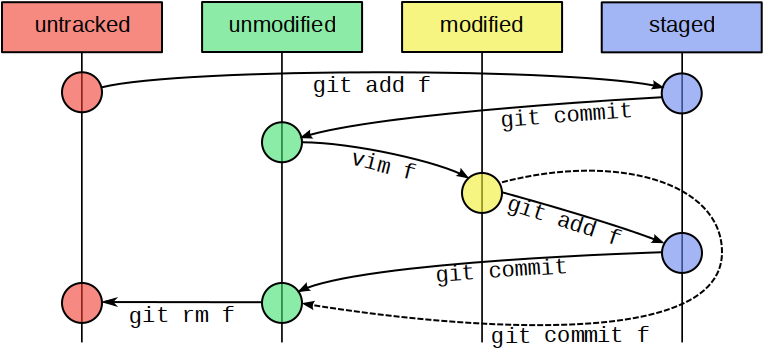
\includegraphics[scale = 0.55]{resources/git_workflow.png}
   \caption{Basic git workflow}
\end{figure}

\subsubsection{One last thing}

Remember when we said that git was a distributed tool that allowed people to collaborate on the same project? We have not covered that part.

Actually, commits can be synchronized with a server. We will not cover it in details at all; for now you just need to now that if your git repository exists on a remote server you can \textbf{push} your tree to make your commits available to other collaborators and \textbf{pull} the latest commits made by other collaborators. The respective commands to perform these two actions are, surprisingly, \texttt{git push} and \texttt{git pull}.

Think of it as a Google doc where you write stuff collaboratively: when you make changes, everybody can see them and when other make changes, you can see them. When you write code as a member of a team, you also want to share your code with your teammates and retrieve code changes from your teammates; most teams do it with git.

\section{Practical exercises}

%You have been created an account and a custom repository on a \href{https://gitea.electrosenpai.dev}{Gitea server}. You will use it to play with git by yourself.
We are going to use the popular "development platform" \href{https://github.com/}{Github}. This platform is the leader in the industry and millions of developers use it. Most engineering teams use either GitHub or a similar platform on a daily basis.

\subsection{Getting access}

\subsubsection{Create an account}

Create an account there and verificate it by confirming your email. Make sure you use the same email you used to configure git.

\subsubsection{Setup SSH}

The preferred way to communicate with a git remote (understand \textit{a repository online}) is through SSH. SSH is a protocol providing a secure communication channel between two hosts. It relies on symmetric and asymmetric cryptography.

We are not going to dig into the details of that protocol as it would be out of scope for that tutorial. Instead, remember that we need to generate a private (\textbf{secret}) key and a public (\textbf{not secret}) key and to communicate the public key to the git server.
The following command will generate a 4096 bits RSA keypair:

\begin{lstlisting}[language=bash]
$ssh-keygen -t rsa -b 4096
Generating public/private rsa key pair.
Enter file in which to save the key (/home/nicolas/.ssh/id_rsa): # Do not put anything here, it is the right place
Enter passphrase (empty for no passphrase): 
Enter same passphrase again:
Your identification has been saved in /home/nicolas/.ssh/id_rsa.
Your public key has been saved in /home/nicolas/.ssh/id_rsa.pub.
The key fingerprint is:
SHA256:pUuEbId+QRZgIE4Zu7fI/ZqViyISKJDV9nk4f9cLCh4 nicolas@nicolas-laptop
The key's randomart image is:
+---[RSA 4096]----+
|  ++..o.+.       |
| ooooo =         |
| oo. .=o+ .      |
|o  . o=o.+       |
|o . . .+S    .   |
|+. + . +E.. o .  |
|..o o o..+ o . . |
|o .  = .. .   .  |
|.. .+.o          |
+----[SHA256]-----+
\end{lstlisting}

Following that command, the keys are put in your home, in the hidden folder \texttt{.ssh/}. The public key is the one with the \texttt{.pub} extension. As it is public, it can be shared with anyone without any risk. The private one is the one without extension. You should not touch that file.

Now, display the content of that public key file (you can use \texttt{cat /home/your\_name/.ssh/id\_rsa.pub} to get it). It should look like this:

\begin{lstlisting}[language=bash]
$cat /home/nicolas/.ssh/id_rsa.pub
ssh-rsa AAAAB3NzaC1yc2EAAAADAQABAAACAQDG7B9ZYR5zUgCjSe2VIFHL6K36UCJDzmP4/dgkn6CGcl/40IxYQi6Ynt7wqasuCrLLQMd02MJ6YkofnP9emC3eYWzZ0vrtfhBhQTU1H8Rn5PmQBtfLBBSSe3kwaVVNKSj2GlW6iJaCYzMHXgLJUZl/3henTMKxQAknr5vdXyfAnIbEtQP3UMYpokJS8Y1GA45i55m87CzaMv/jygKn79KXyC8t92G6UWpfxgc/LbW7Myo0P1yeMeK8c2d3zkeCqQtiDoxHSQpDq4ULYErKrfeLHTXosKs/fgpti7TG16P88r/WIavqMCWrHEimHzw/qNRmHGD+VAQOw0Il/CydykhZLGW4NgVr4gAoCejhqTHxOTeuGbJWNo3tPTEubbMiT1vDOKb5/qqH5dNdv8vSU4uMvyfe5qaJtPHwHg2BX4aOqjJ1Cqyy9p4LY5cBFwv4Qt9HiR2ApgOynErnetwzD236XZLl/LdaXT83SRaqn7wk5uTRUQq0VSY4/eyxERoKF+aKARmr2OIgYbrvkouZybWpjH6Tr8dBJw9FMsLRJ+ZPuk57vAaGqXVf1fdg4IC8BahRJQhImkfiyvjg0cOMUuZPzeGU1mIxGCOmMJRaWr79oH8pqZL5a/cc2B8hD9DEGF3421mrYMYqSoWzgjqs7hTuwz+Bes/4zTCoTatClXJrrw== nicolas@Nicolass-MacBook-Pro.local
\end{lstlisting}

Then, copy it and put it in Github: go to \href{github.com}{github.com}, click on your profile picture at the top right, browse \textit{Settings}, \textit{SSH and GPG Keys}, \textit{New SSH keys}.

The field \textit{Title} does not matter. Paste the key in \textit{Content}.

\subsection{Try out commands!}

\subsubsection{Create a new repository}

Create a new repository: navigate to \href{https://github.com/new}{https://github.com/new} and write down \texttt{git-tutorial} as the name of the repository. Set the repository visibility to \textbf{Public}. Make sure you put the right name there!

If you completed the previous section correctly, you should be able to clone the repository you just created in your workstation.
Open a terminal and run the following command:

\texttt{git clone git@github.com:YOUR\_USERNAME\_HERE/git-tutorial.git}

You will be prompted for the SSH passphrase you may have entered before. Enter it, press enter and use \texttt{ls}... You should see a new directory there! It is the git repository that you just created.

\begin{lstlisting}[language=bash]
$git clone git@github.com:nicoche/git-tutorial.git
Cloning into 'git-tutorial...
The authenticity of host '[github.com]:443 ([IP]:443)' can't be established.
ECDSA key fingerprint is SHA256:...
Are you sure you want to continue connecting (yes/no)? yes
Warning: Permanently added '[github.com]:443 ([IP]:443)' (ECDSA) to the list of known hosts.
remote: Enumerating objects: 3, done.
remote: Countring objects: 100\% (3/3), done.
remote: Total 3 (delta 0), reused 0 (delta 0)
Receiving objects: 100\% (3/3), done.
$ls
git-tutorial
$cd git-tutorial
$git status
On branch master

No commits yet

nothing to commit (create/copy files and use "git add" to track)
\end{lstlisting}

\subsubsection{Exercise}

You now have everything you need. We will not work on in-depth exercises as we only covered the basics of git but you now should be able to versionate code and push it to a repository.

Feel free to play around with git, but in the end, your repository needs to meet the following requirements:

\begin{itemize}
	\item Contain three distinct commits, each of them containg a new empty file. They should be named \texttt{empty\_file\_1}, \texttt{empty\_file\_2} and \texttt{empty\_file\_3}. Note that they must be created in \textbf{distinct} commits
	\item Contain a commit that creates a new file called \texttt{README.md}. It should contain your first name, a space and then your last name
	\item Contain a commit that creates a new file called \texttt{modify\_me.txt}. It should contain the text \textit{2 + 2 = 5}
	\item Contain a commit that modifies the file called \texttt{modify\_me.txt} from \textit{2 + 2 = 5} to \textit{2 + 2 = 4}
	\item Bonus: put the code from the last section of tutorial 1 in the executable file \texttt{guessing\_game.py} and add features to it. It could be anything, from asking the name of the player and displaying it when he wins, to restricting the number of guesses the player can make. For each feature, make a commit
\end{itemize}

Pay attention to the following points:

\begin{itemize}
	\item All commits must be made via the command line
	\item You need to push your commits to GitHub with the command \texttt{git push}. You can do it at any time and repeat it whenever you want. After a successful push, you can visit the repository page at \href{https://github.com/YOUR\_USERNAME\_HERE/git-tutorial}{https://github.com/YOUR\_USERNAME\_HERE/git-tutorial}
	\item At any time, use \texttt{git status} to know what the current status of the repository is. Use \texttt{git log} to see the history of commits
	\item This exercise will be automatically corrected so \textbf{the spaces and filenames are important}. Files with the wrong name will be ignored!
\end{itemize}

\end{document}
